%----------------------------------------------------------------------------------------
%    PACKAGES AND THEMES
%----------------------------------------------------------------------------------------

\documentclass[aspectratio=169,xcolor=dvipsnames]{beamer}
\usetheme{SimpleDarkBlue}

\usepackage{hyperref}
\usepackage{graphicx}
\usepackage{booktabs}
\usepackage{tikz}
\usetikzlibrary{positioning,arrows}
\usepackage{amsmath}
\usepackage{multirow}
\usepackage{adjustbox}
\usepackage{colortbl}

%----------------------------------------------------------------------------------------
%    TITLE PAGE
%----------------------------------------------------------------------------------------

\title{SarcasmLens: Subjective Sarcasm Detection in Hindi-English Code-Mixed Social Media Text}

\author{Jash Shah - 202201016@dau.ac.in}

\institute
{
    Dhirubhai Ambani University
}
\date{\today}

%----------------------------------------------------------------------------------------
%    PRESENTATION SLIDES
%----------------------------------------------------------------------------------------

\begin{document}

% Title
\begin{frame}
    \titlepage
\end{frame}

%----------------------------------------------------------------------------------------
% SLIDE 1: Problem and Motivation
%----------------------------------------------------------------------------------------

\section{Problem and Motivation}

\begin{frame}{Problem and Motivation}
    \textbf{Challenge}: Sarcasm detection in Hindi-English code-mixed social media text
    
    \begin{itemize}
        \item \textbf{Code-mixing}: Seamless blending of Hindi and English within single utterances
        \item \textbf{Transliteration variations}: Inconsistent spelling (e.g., ``kya'', ``kiya'', ``kiyaa'')
        \item \textbf{Cultural context}: References to Indian politics, entertainment, social issues
        \item \textbf{Informal language}: Social media slang and abbreviations
    \end{itemize}
    
    \vspace{0.3cm}
    
    \textbf{Why It Matters}:
    \begin{itemize}
        \item Millions of code-mixed posts daily on Indian social media
        \item Critical for sentiment analysis, brand monitoring, content moderation
        \item Traditional monolingual systems fail to capture code-mixing nuances
    \end{itemize}
\end{frame}

%----------------------------------------------------------------------------------------
% SLIDE 2: Data Modelling - Dataset + Preprocessing
%----------------------------------------------------------------------------------------

\section{Data Modelling}

\begin{frame}{Dataset \& Preprocessing}
    \begin{columns}
        \column{0.5\textwidth}
        \textbf{Combined Corpus: 15,099 samples}
        \begin{itemize}
            \item Swami et al. (2018)
            \item HackArena Dataset
            \item Mendeley Dataset
            \item Aggarwal et al. (2020)
        \end{itemize}
        
        \vspace{0.3cm}
        
        \textbf{Statistics}
        \begin{itemize}
            \item Non-sarcastic: 8,091 (53.6\%)
            \item Sarcastic: 7,008 (46.4\%)
            \item Mean length: 80.89 chars
        \end{itemize}
        
        \column{0.5\textwidth}
        \textbf{7-Step Preprocessing}
        \begin{enumerate}
            \item Lowercasing
            \item Remove @ mentions
            \item Hashtag processing
            \item URL removal
            \item Punctuation removal
            \item Stop word removal (English only)
            \item Whitespace normalization
        \end{enumerate}
        
        \vspace{0.3cm}
        
        \textbf{Example}:
        \begin{itemize}
            \item \textit{Before}: @user123 Kya aapko lagta hai ki yeh brilliant idea hai?
            \item \textit{After}: kya aapko lagta hai ki yeh brilliant idea hai
        \end{itemize}
    \end{columns}
\end{frame}

%----------------------------------------------------------------------------------------
% SLIDE 3: Methodology/Pipeline - Workflow
%----------------------------------------------------------------------------------------

\section{Methodology}

\begin{frame}{System Pipeline}
    \begin{center}
        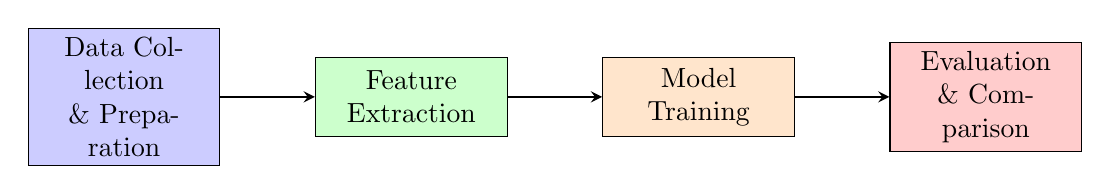
\begin{tikzpicture}[node distance=1.2cm, auto, >=stealth]
            \node[rectangle, draw, fill=blue!20, text width=2.2cm, align=center, minimum height=1cm] (data) {Data Collection\\ \& Preparation};
            \node[rectangle, draw, fill=green!20, text width=2.2cm, align=center, minimum height=1cm, right=of data] (features) {Feature\\ Extraction};
            \node[rectangle, draw, fill=orange!20, text width=2.2cm, align=center, minimum height=1cm, right=of features] (train) {Model\\ Training};
            \node[rectangle, draw, fill=red!20, text width=2.2cm, align=center, minimum height=1cm, right=of train] (eval) {Evaluation\\ \& Comparison};
            
            \draw[->, thick] (data) -- (features);
            \draw[->, thick] (features) -- (train);
            \draw[->, thick] (train) -- (eval);
        \end{tikzpicture}
    \end{center}
    
    \vspace{0.5cm}
    
    \textbf{Four Phases}:
    \begin{enumerate}
        \item \textbf{Data Collection}: Combine 4 datasets → 15,099 samples
        \item \textbf{Feature Extraction}: TF-IDF, FastText, BiLSTM tokenization, Transformer tokenization
        \item \textbf{Model Training}: Train 8 different models with stratified 80/20 split
        \item \textbf{Evaluation}: Compare performance using accuracy, F1, precision, recall
    \end{enumerate}
\end{frame}

%----------------------------------------------------------------------------------------
% SLIDE 4: Model Framework - Architecture, algorithms
%----------------------------------------------------------------------------------------

\section{Model Framework}

\begin{frame}{Model Architectures \& Design Choices}
    \begin{columns}
        \column{0.5\textwidth}
        \textbf{Traditional ML}
        \begin{itemize}
            \item TF-IDF + RF/SVM
            \item FastText + RF/SVM
        \end{itemize}
        
        \vspace{0.3cm}
        
        \textbf{Deep Learning}
        \begin{itemize}
            \item BiLSTM: Embedding(128) → BiLSTM(64) → Dense(1)
        \end{itemize}
        
        \vspace{0.3cm}
        
        \textbf{Transformers}
        \begin{itemize}
            \item XLM-RoBERTa-base
            \item mBERT
            \item Indic-BERT
        \end{itemize}
        
        \column{0.5\textwidth}
        \textbf{FastText Advantages}
        \begin{itemize}
            \item Character n-grams handle OOV words
            \item Captures transliteration variations
            \item Better for code-mixed text
        \end{itemize}
        
        \vspace{0.3cm}
        
        \textbf{Random Forest Benefits}
        \begin{itemize}
            \item Non-linear decision boundaries
            \item Ensemble averaging
            \item Handles class imbalance
        \end{itemize}
        
        \vspace{0.3cm}
        
        \textbf{Best Combination}: FastText embeddings + Random Forest classifier
    \end{columns}
\end{frame}

%----------------------------------------------------------------------------------------
% SLIDE 5: Evaluation Setup
%----------------------------------------------------------------------------------------

\section{Evaluation Setup}

\begin{frame}{Evaluation Metrics}
    \begin{columns}
        \column{0.5\textwidth}
        \textbf{Metrics}
        \begin{itemize}
            \item \textbf{Accuracy}: Overall correctness
            \item \textbf{Precision}: $\frac{TP}{TP+FP}$
            \item \textbf{Recall}: $\frac{TP}{TP+FN}$
            \item \textbf{F1 Score}: Harmonic mean
        \end{itemize}
        
        \column{0.5\textwidth}
        \textbf{Experimental Setup}
        \begin{itemize}
            \item \textbf{Split}: Stratified 80/20 train/test
            \item \textbf{Seed}: 42 (reproducibility)
            \item \textbf{Class weights}: Balanced handling
            \item \textbf{Test set}: 3,020 samples
        \end{itemize}
    \end{columns}
    
    \vspace{0.3cm}
    
    \textbf{Baselines}: TF-IDF + RF/SVM, FastText + RF/SVM, BiLSTM, XLM-RoBERTa, mBERT, Indic-BERT
\end{frame}

%----------------------------------------------------------------------------------------
% SLIDE 6: Results - Key tables, insights
%----------------------------------------------------------------------------------------

\section{Results}

\begin{frame}{Results \& Key Insights}
    \begin{center}
        \small
        \adjustbox{width=0.6\textwidth,center}{
        \begin{tabular}{lcccc}
        \toprule
        \textbf{Model} & \textbf{Acc.} & \textbf{F1} & \textbf{Prec.} & \textbf{Rec.} \\
        \midrule
        TF-IDF + RF & 0.9755 & 0.9755 & 0.9754 & 0.9756 \\
        TF-IDF + SVM & 0.9762 & 0.9762 & 0.9761 & 0.9763 \\
        \rowcolor{green!20}
        \textbf{FastText + RF} & \textbf{0.9772} & \textbf{0.9771} & \textbf{0.9779} & 0.9772 \\
        FastText + SVM & 0.9493 & 0.9492 & 0.9509 & 0.9493 \\
        BiLSTM & 0.9705 & 0.9705 & 0.9704 & 0.9706 \\
        XLM-RoBERTa & 0.9669 & 0.9652 & 0.9429 & 0.9886 \\
        mBERT & 0.9609 & 0.9587 & 0.9421 & 0.9757 \\
        Indic-BERT & 0.9649 & 0.9633 & 0.9355 & \textbf{0.9929} \\
        \bottomrule
        \end{tabular}
        }
    \end{center}
    
    \vspace{0.2cm}
    
    \begin{columns}
        \column{0.5\textwidth}
        \textbf{Key Findings}
        \begin{itemize}
            \item All models $>$94\% accuracy
            \item FastText + RF: \textbf{97.72\%} accuracy
            \item FastText beats TF-IDF
            \item RF beats SVM (non-linear)
        \end{itemize}
        
        \column{0.5\textwidth}
        \textbf{Transformer Performance}
        \begin{itemize}
            \item XLM-RoBERTa: 96.69\% accuracy
            \item High recall ($>$97\%)
            \item Indic-BERT: 99.29\% recall
        \end{itemize}
    \end{columns}
\end{frame}

%----------------------------------------------------------------------------------------
% SLIDE 7: Conclusion
%----------------------------------------------------------------------------------------

\section{Conclusion}

\begin{frame}{Conclusion}
    \textbf{Key Contributions}
    \begin{itemize}
        \item Unified corpus: 15,099 samples from 4 datasets
        \item Systematic comparison of 8 models across 4 categories
        \item Best model: FastText + Random Forest (97.72\% accuracy)
        \item Demonstrates effectiveness of subword-aware embeddings for code-mixed text
    \end{itemize}
    
    \vspace{0.3cm}
    
    \textbf{Key Findings}
    \begin{itemize}
        \item FastText embeddings outperform TF-IDF for code-mixed sarcasm detection
        \item Non-linear classifiers (Random Forest) better than linear (SVM)
        \item Transformer models achieve competitive performance ($>$96\% accuracy)
        \item Practical solution: Fast training + high accuracy
    \end{itemize}
    
    \vspace{0.3cm}
    
    \textbf{Future Work}: Error analysis, cross-dataset generalization, feature engineering, model interpretability, real-world deployment
\end{frame}

\end{document}

